\chapter{Unified Modeling Language: Behavioral Diagrams}

\section{Pendahuluan}


\section{Behavioral Diagram}

Behavioral diagram merupakan jenis diagram dalam Unified Modeling Language (UML) yang digunakan untuk merepresentasikan dinamika dan interaksi dalam suatu sistem perangkat lunak. Diagram ini menggambarkan bagaimana komponen dalam sistem beroperasi, bagaimana aliran data atau informasi terjadi, serta bagaimana objek berinteraksi satu sama lain selama eksekusi. Behavioral diagram sangat berguna dalam memahami alur kerja sistem sebelum implementasi, terutama dalam konteks analisis kebutuhan dan desain perangkat lunak.

Terdapat beberapa jenis behavioral diagram dalam UML, termasuk sequence diagram, activity diagram, state machine diagram, dan use case diagram. Masing-masing diagram memiliki peran yang berbeda dalam mendokumentasikan perilaku sistem.


\section{Activity Diagram}

Activity diagram merupakan salah satu diagram perilaku dalam Unified Modeling Language (UML) yang digunakan untuk merepresentasikan aliran proses dalam suatu sistem perangkat lunak. Diagram ini menggambarkan langkah-langkah yang dilakukan dalam sistem, termasuk percabangan, perulangan, eksekusi paralel, serta penanganan kesalahan. Berikut adalah fitur-fitur utama dalam activity diagram:


\begin{figure}[ht]
		\centering
		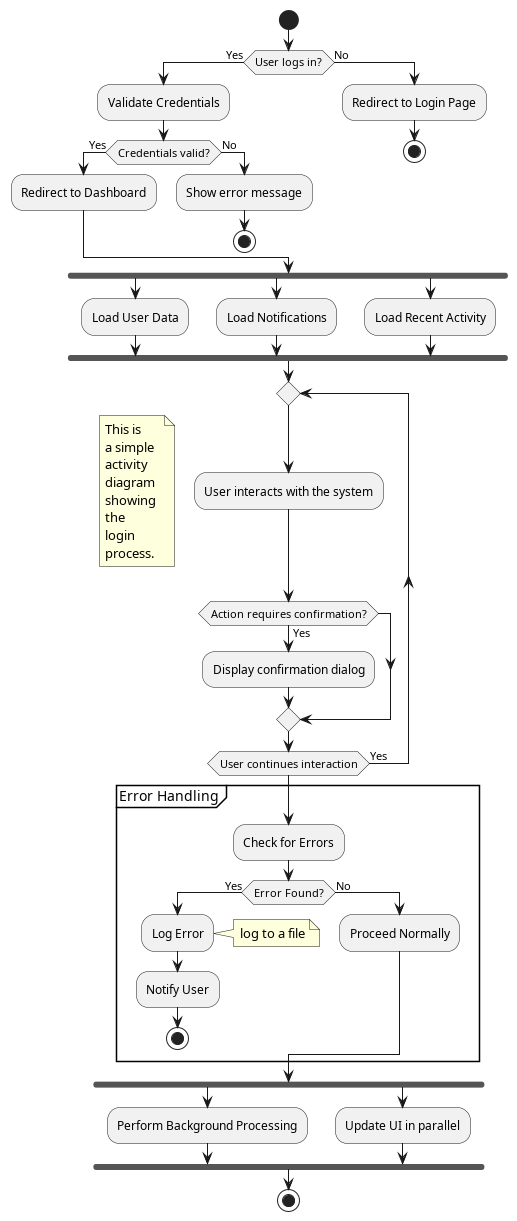
\includegraphics[width=.44\textwidth]{../figures/out/activity_diagram}
		\caption{Activity diagram and its features}
		\label{fig:activity_diagram}
\end{figure}

\begin{lstlisting}[language=puml, caption=PlantUML code for the activity diagram.]
@startuml

start

' Decision Node
if (User logs in?) then (Yes)
:Validate Credentials;
if (Credentials valid?) then (Yes)
:Redirect to Dashboard;
else (No)
:Show error message;
stop
endif
else (No)
:Redirect to Login Page;
stop
endif

' Fork Node - Parallel Execution
fork
:Load User Data;
fork again
:Load Notifications;
fork again
:Load Recent Activity;
end fork

' Looping Construct
repeat
:User interacts with the system;
floating note left
This is 
a simple 
activity 
diagram
showing 
the 
login 
process.
end note
if (Action requires confirmation?) then (Yes)
:Display confirmation dialog;
endif
repeat while (User continues interaction) is (Yes)

' Exception Handling
partition "Error Handling" {
	:Check for Errors;
	if (Error Found?) then (Yes)
	:Log Error;
	' Notes explaining components
	note right
	log to a file
	end note
	:Notify User;
	stop
	else (No)
	:Proceed Normally;
	endif
}

' Synchronization and Merging Flows
fork
:Perform Background Processing;
fork again
:Update UI in parallel;
end fork

' Final Node
stop

@enduml
\end{lstlisting}


\subsection{Alur Masuk dan Keputusan}
Activity diagram dimulai dengan \textit{start node} yang merepresentasikan awal proses sistem. Langkah pertama dalam diagram ini adalah memeriksa apakah pengguna sudah masuk (\texttt{User logs in?}). Jika ya, sistem akan memvalidasi kredensial pengguna:

\begin{lstlisting}[language=puml]
	if (User logs in?) then (Yes)
	:Validate Credentials;
	if (Credentials valid?) then (Yes)
	:Redirect to Dashboard;
	else (No)
	:Show error message;
	stop
	endif
	else (No)
	:Redirect to Login Page;
	stop
	endif
\end{lstlisting}

Jika kredensial valid, pengguna akan diarahkan ke halaman dashboard. Jika tidak valid, sistem menampilkan pesan kesalahan dan menghentikan eksekusi. Jika pengguna tidak masuk, sistem akan mengarahkannya ke halaman login.

\subsection{Eksekusi Paralel}
Activity diagram mendukung eksekusi paralel menggunakan \textit{fork node}. Hal ini memungkinkan beberapa aktivitas dijalankan bersamaan sebelum akhirnya disinkronisasi kembali. Dalam diagram ini, setelah pengguna berhasil masuk, sistem akan memuat data pengguna, notifikasi, dan aktivitas terbaru secara paralel:

\begin{lstlisting}[language=puml]
	fork
	:Load User Data;
	fork again
	:Load Notifications;
	fork again
	:Load Recent Activity;
	end fork
\end{lstlisting}

Proses ini meningkatkan efisiensi karena sistem dapat menangani beberapa tugas sekaligus.

\subsection{Perulangan}
Perulangan dalam activity diagram direpresentasikan menggunakan struktur \texttt{repeat}, yang memungkinkan sistem untuk mengulang suatu aktivitas hingga kondisi tertentu tidak lagi terpenuhi. Contoh dalam diagram adalah interaksi pengguna dengan sistem yang dapat berulang selama pengguna masih aktif:

\begin{lstlisting}[language=puml]
	repeat
	:User interacts with the system;
	floating note left
	This is 
	a simple 
	activity 
	diagram
	showing 
	the 
	login 
	process.
	end note
	if (Action requires confirmation?) then (Yes)
	:Display confirmation dialog;
	endif
	repeat while (User continues interaction) is (Yes)
\end{lstlisting}

Pengguna dapat terus berinteraksi dengan sistem hingga mereka berhenti menggunakan aplikasi.

\subsection{Penanganan Kesalahan}
Activity diagram juga dapat merepresentasikan mekanisme penanganan kesalahan (\textit{error handling}). Dalam contoh diagram, jika terjadi kesalahan, sistem akan mencatat log kesalahan dan memberi tahu pengguna:

\begin{lstlisting}[language=puml]
	partition "Error Handling" {
		:Check for Errors;
		if (Error Found?) then (Yes)
		:Log Error;
		note right
		log to a file
		end note
		:Notify User;
		stop
		else (No)
		:Proceed Normally;
		endif
	}
\end{lstlisting}

Sistem memeriksa apakah ada kesalahan. Jika ada, sistem mencatatnya dalam log dan memberi tahu pengguna sebelum menghentikan proses.

\subsection{Sinkronisasi dan Penggabungan Aliran}
Selain eksekusi paralel, activity diagram mendukung \textit{join node} untuk menyinkronisasi aktivitas yang berjalan bersamaan. Dalam contoh diagram, setelah proses latar belakang selesai, sistem memperbarui UI:

\begin{lstlisting}[language=puml]
	fork
	:Perform Background Processing;
	fork again
	:Update UI in parallel;
	end fork
\end{lstlisting}

Hal ini memastikan bahwa pemrosesan berjalan secara efisien tanpa mengganggu tampilan antarmuka pengguna.

\subsection{Node Awal dan Akhir}
Activity diagram selalu memiliki titik awal (\textit{start node}) dan titik akhir (\textit{stop node}) untuk menandai awal dan akhir dari proses. Pada diagram ini, alur dimulai dengan:

\begin{lstlisting}[language=puml]
	start
\end{lstlisting}

Dan berakhir dengan:

\begin{lstlisting}[language=puml]
	stop
\end{lstlisting}

\subsection{Catatan dalam Diagram}
Dalam UML, catatan (\textit{notes}) digunakan untuk memberikan informasi tambahan tentang elemen dalam diagram. Contoh catatan dalam diagram adalah:

\begin{lstlisting}[language=puml]
	floating note left
	This is 
	a simple 
	activity 
	diagram
	showing 
	the 
	login 
	process.
	end note
\end{lstlisting}

Catatan ini memberikan konteks bagi pembaca untuk memahami bagaimana proses login bekerja dalam sistem.

Activity diagram sangat berguna dalam pemodelan perangkat lunak karena memungkinkan pengembang memahami alur eksekusi sistem sebelum implementasi. Diagram ini mencakup berbagai elemen seperti aktivitas, keputusan, eksekusi paralel, perulangan, penanganan kesalahan, serta catatan tambahan untuk dokumentasi yang lebih jelas.


\section{Sequence Diagram}

Sequence diagram merupakan salah satu diagram perilaku dalam Unified Modeling Language (UML) yang digunakan untuk memodelkan interaksi antar objek dalam suatu sistem secara berurutan. Diagram ini menggambarkan bagaimana pesan dikirim dan diterima antar partisipan dalam suatu skenario tertentu. Sequence diagram sangat berguna dalam memahami bagaimana suatu fitur atau proses bekerja secara detail dengan memperlihatkan alur komunikasi antar komponen dalam sistem. Berikut adalah fitur-fitur utama dalam sequence diagram.

\begin{figure}[ht]
	\centering
	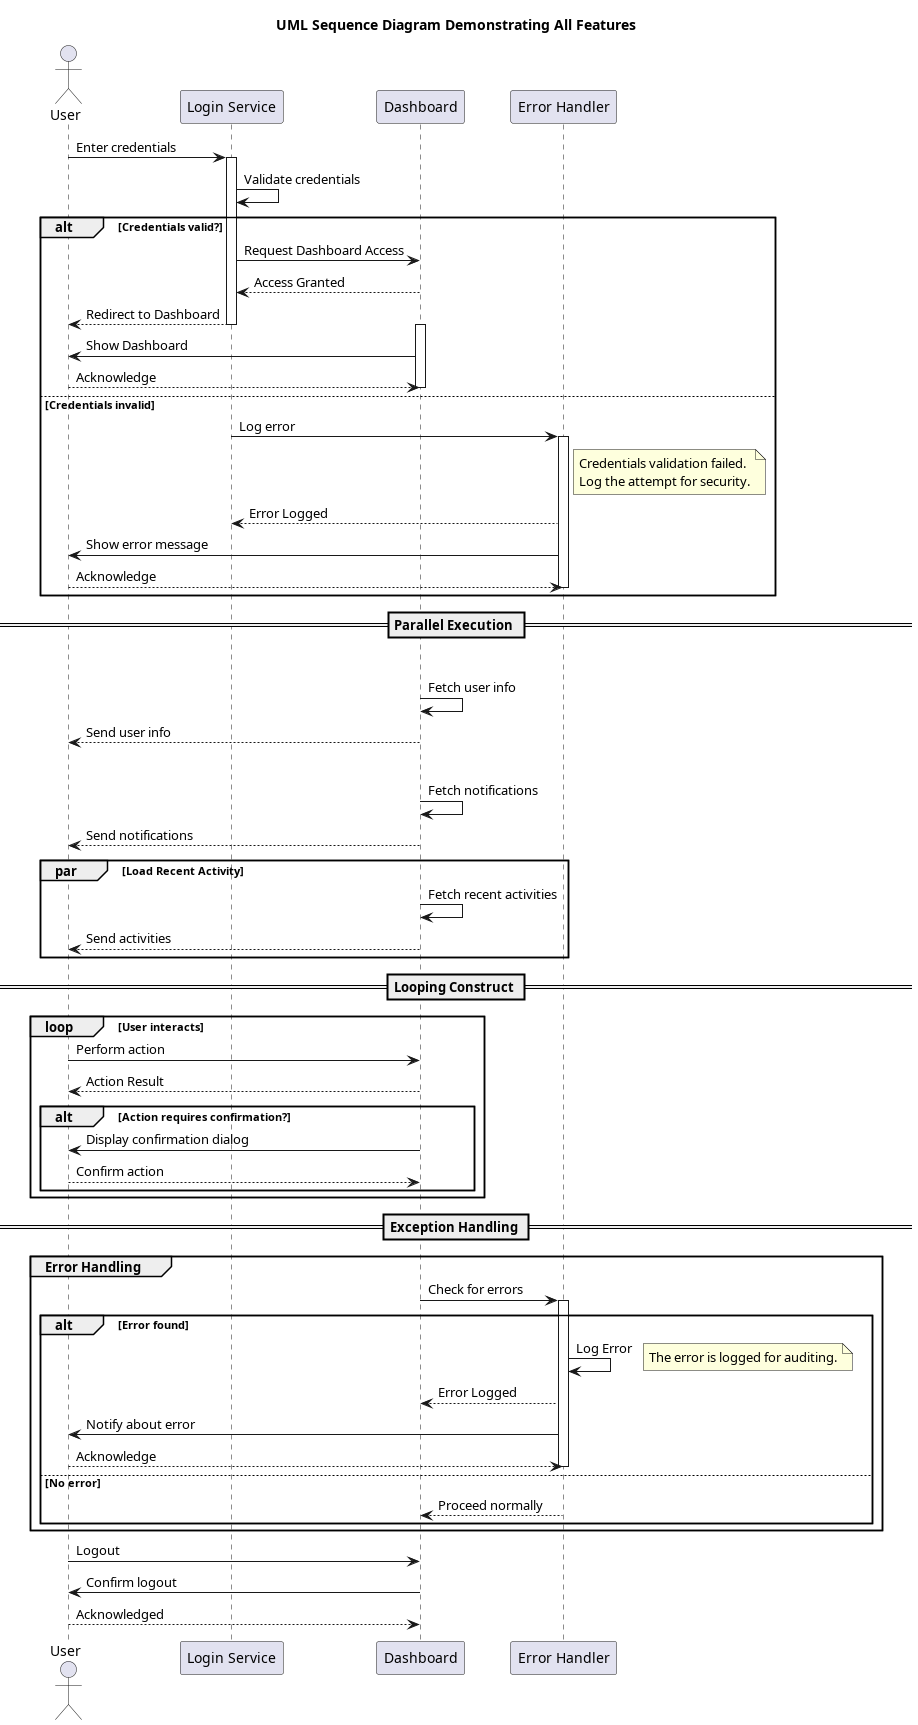
\includegraphics[width=.55\textwidth]{../figures/out/sequence_diagram}
	\caption{Sequence diagram and its features}
	\label{fig:sequence_diagram}
\end{figure}

\begin{lstlisting}[language=puml, caption=PlantUML code for the sequence diagram.]
@startuml
title UML Sequence Diagram Demonstrating All Features

actor User
participant "Login Service" as LS
participant "Dashboard" as DB
participant "Error Handler" as EH

User -> LS: Enter credentials
activate LS
LS -> LS: Validate credentials

alt Credentials valid?
LS -> DB: Request Dashboard Access
DB --> LS: Access Granted
LS --> User: Redirect to Dashboard
deactivate LS
else Credentials invalid
LS -> EH: Log error
activate EH
note right of EH
Credentials validation failed.
Log the attempt for security.
end note
EH --> LS: Error Logged
EH -> User: Show error message
User --> EH: Acknowledge
deactivate EH
deactivate LS
end alt

== Parallel Execution ==
par Load User Data
DB -> DB: Fetch user info
DB --> User: Send user info
par Load Notifications
DB -> DB: Fetch notifications
DB --> User: Send notifications
par Load Recent Activity
DB -> DB: Fetch recent activities
DB --> User: Send activities
end par

== Looping Construct ==
loop User interacts
User -> DB: Perform action
DB --> User: Action Result
alt Action requires confirmation?
DB -> User: Display confirmation dialog
User --> DB: Confirm action
end alt
end loop

== Exception Handling ==
group Error Handling
DB -> EH: Check for errors
activate EH
alt Error found
EH -> EH: Log Error
note right
The error is logged for auditing.
end note
EH --> DB: Error Logged
EH -> User: Notify about error
User --> EH: Acknowledge
deactivate EH
else No error
EH --> DB: Proceed normally
end alt
end group

User -> DB: Logout
DB -> User: Confirm logout
User --> DB: Acknowledged
deactivate DB

@enduml
\end{lstlisting}

\subsection{Aktor dan Partisipan}
Aktor dan partisipan dalam sequence diagram merepresentasikan entitas yang terlibat dalam interaksi sistem. Aktor biasanya merupakan pengguna atau sistem eksternal, sedangkan partisipan adalah komponen internal yang menerima dan mengirim pesan. Dalam contoh diagram ini, terdapat aktor \texttt{User} yang berinteraksi dengan beberapa partisipan, yaitu \texttt{Login Service}, \texttt{Dashboard}, dan \texttt{Error Handler}.

Deklarasi aktor dan partisipan dalam PlantUML dilakukan menggunakan sintaks berikut:
\begin{lstlisting}[language=puml]
	actor User
	participant "Login Service" as LS
	participant "Dashboard" as DB
	participant "Error Handler" as EH
\end{lstlisting}
Aktor dan partisipan ini menentukan siapa yang akan mengirim dan menerima pesan dalam diagram.

\subsection{Pengiriman Pesan}
Pesan dalam sequence diagram merepresentasikan komunikasi antara partisipan. Terdapat dua jenis pesan yang digunakan dalam diagram ini. Pesan sinkron menggunakan panah solid (\texttt{->}) yang menunjukkan bahwa pemanggil harus menunggu respons sebelum melanjutkan eksekusi. Pesan balik direpresentasikan dengan panah putus-putus (\texttt{-->}), menandakan bahwa suatu partisipan mengembalikan hasil pemrosesan kepada pemanggil.

Pada awal interaksi, pengguna mengirimkan kredensial login ke \texttt{Login Service} untuk divalidasi. Jika kredensial valid, layanan ini akan mengirim permintaan akses ke \texttt{Dashboard}, dan setelah menerima respons, pengguna akan diarahkan ke tampilan utama. Jika kredensial tidak valid, sistem akan mencatat kesalahan dan menampilkan pesan peringatan kepada pengguna.

\begin{lstlisting}[language=puml]
	User -> LS: Enter credentials
	LS -> LS: Validate credentials
	LS -> DB: Request Dashboard Access
	DB --> LS: Access Granted
	LS --> User: Redirect to Dashboard
\end{lstlisting}

\subsection{Aktivasi dan Deaktivasi}
Aktivasi dalam sequence diagram menunjukkan bahwa suatu objek sedang menjalankan suatu proses. Aktivasi terjadi setelah objek menerima pesan dan akan bertahan hingga objek menyelesaikan tugasnya. Aktivasi ditandai dengan perintah \texttt{activate} untuk menunjukkan bahwa suatu partisipan sedang aktif menjalankan suatu proses, dan \texttt{deactivate} untuk menandakan bahwa partisipan telah menyelesaikan tugasnya.

Dalam contoh diagram ini, \texttt{Login Service} diaktifkan ketika menerima permintaan login dan tetap aktif selama memvalidasi kredensial. Setelah proses selesai, partisipan ini dinonaktifkan.

\begin{lstlisting}[language=puml]
	activate LS
	LS -> LS: Validate credentials
	deactivate LS
\end{lstlisting}

\subsection{Percabangan (\texttt{alt})}
PlantUML menyediakan blok \texttt{alt} untuk menangani percabangan dalam suatu alur proses. Percabangan ini digunakan untuk merepresentasikan keputusan dalam sistem, seperti validasi kredensial pengguna.

Dalam contoh diagram ini, jika kredensial valid, sistem akan mengarahkan pengguna ke \texttt{Dashboard}. Sebaliknya, jika kredensial tidak valid, sistem akan mencatat kesalahan dan menampilkan pesan kesalahan.

\begin{lstlisting}[language=puml]
	alt Credentials valid?
	LS -> DB: Request Dashboard Access
	DB --> LS: Access Granted
	LS --> User: Redirect to Dashboard
	else Credentials invalid
	LS -> EH: Log error
	EH --> LS: Error Logged
	EH -> User: Show error message
	User --> EH: Acknowledge
	end alt
\end{lstlisting}

\subsection{Eksekusi Paralel (\texttt{par})}
Sequence diagram juga mendukung eksekusi paralel dengan menggunakan blok \texttt{par}. Dalam contoh diagram ini, setelah pengguna berhasil login, sistem memuat beberapa informasi secara bersamaan, termasuk data pengguna, notifikasi, dan aktivitas terbaru. Masing-masing tugas ini berjalan secara independen tanpa saling menunggu.

\begin{lstlisting}[language=puml]
	par Load User Data
	DB -> DB: Fetch user info
	DB --> User: Send user info
	par Load Notifications
	DB -> DB: Fetch notifications
	DB --> User: Send notifications
	par Load Recent Activity
	DB -> DB: Fetch recent activities
	DB --> User: Send activities
	end par
\end{lstlisting}

\subsection{Perulangan (\texttt{loop})}
PlantUML menyediakan blok \texttt{loop} untuk merepresentasikan aktivitas yang berulang. Dalam contoh diagram ini, pengguna dapat terus berinteraksi dengan sistem selama sesi masih aktif. Jika suatu aksi memerlukan konfirmasi, sistem akan meminta pengguna untuk mengonfirmasi tindakan tersebut sebelum melanjutkan.

\begin{lstlisting}[language=puml]
	loop User interacts
	User -> DB: Perform action
	DB --> User: Action Result
	alt Action requires confirmation?
	DB -> User: Display confirmation dialog
	User --> DB: Confirm action
	end alt
	end loop
\end{lstlisting}

\subsection{Penanganan Kesalahan (\texttt{group})}
PlantUML mendukung mekanisme penanganan kesalahan menggunakan blok \texttt{group}. Dalam contoh ini, jika terjadi kesalahan selama interaksi dengan sistem, layanan akan mencatat kesalahan dan memberikan notifikasi kepada pengguna.

\begin{lstlisting}[language=puml]
	group Error Handling
	DB -> EH: Check for errors
	activate EH
	alt Error found
	EH -> EH: Log Error
	EH --> DB: Error Logged
	EH -> User: Notify about error
	User --> EH: Acknowledge
	deactivate EH
	else No error
	EH --> DB: Proceed normally
	end alt
	end group
\end{lstlisting}

\subsection{Akhir Interaksi dan Logout}
Sequence diagram juga mencakup proses logout, yang menunjukkan bagaimana pengguna mengakhiri sesi. Setelah logout, sistem akan mengonfirmasi bahwa pengguna telah keluar sebelum mengakhiri interaksi.

\begin{lstlisting}[language=puml]
	User -> DB: Logout
	DB -> User: Confirm logout
	User --> DB: Acknowledged
\end{lstlisting}

Sequence diagram dalam UML sangat berguna untuk memodelkan interaksi antara komponen dalam sistem perangkat lunak. Diagram ini merepresentasikan bagaimana pesan dikirim dan diterima dalam suatu alur proses dengan menampilkan aktor, partisipan, pesan sinkron dan balik, aktivasi, percabangan, eksekusi paralel, perulangan, serta penanganan kesalahan. Dengan menggunakan sequence diagram, pengembang dapat memahami bagaimana sistem bekerja sebelum implementasi dilakukan, memastikan bahwa semua skenario interak



\section{Statechart Diagram}

Statechart diagram merupakan salah satu diagram perilaku dalam Unified Modeling Language (UML) yang digunakan untuk merepresentasikan transisi antara berbagai keadaan (state) dalam suatu sistem. Diagram ini menggambarkan bagaimana sistem berubah dari satu keadaan ke keadaan lain sebagai respons terhadap suatu peristiwa (event) atau kondisi tertentu. Statechart diagram sangat berguna dalam model sistem yang memiliki banyak perubahan status, seperti proses pemesanan dalam e-commerce.

\begin{figure}[ht]
	\centering
	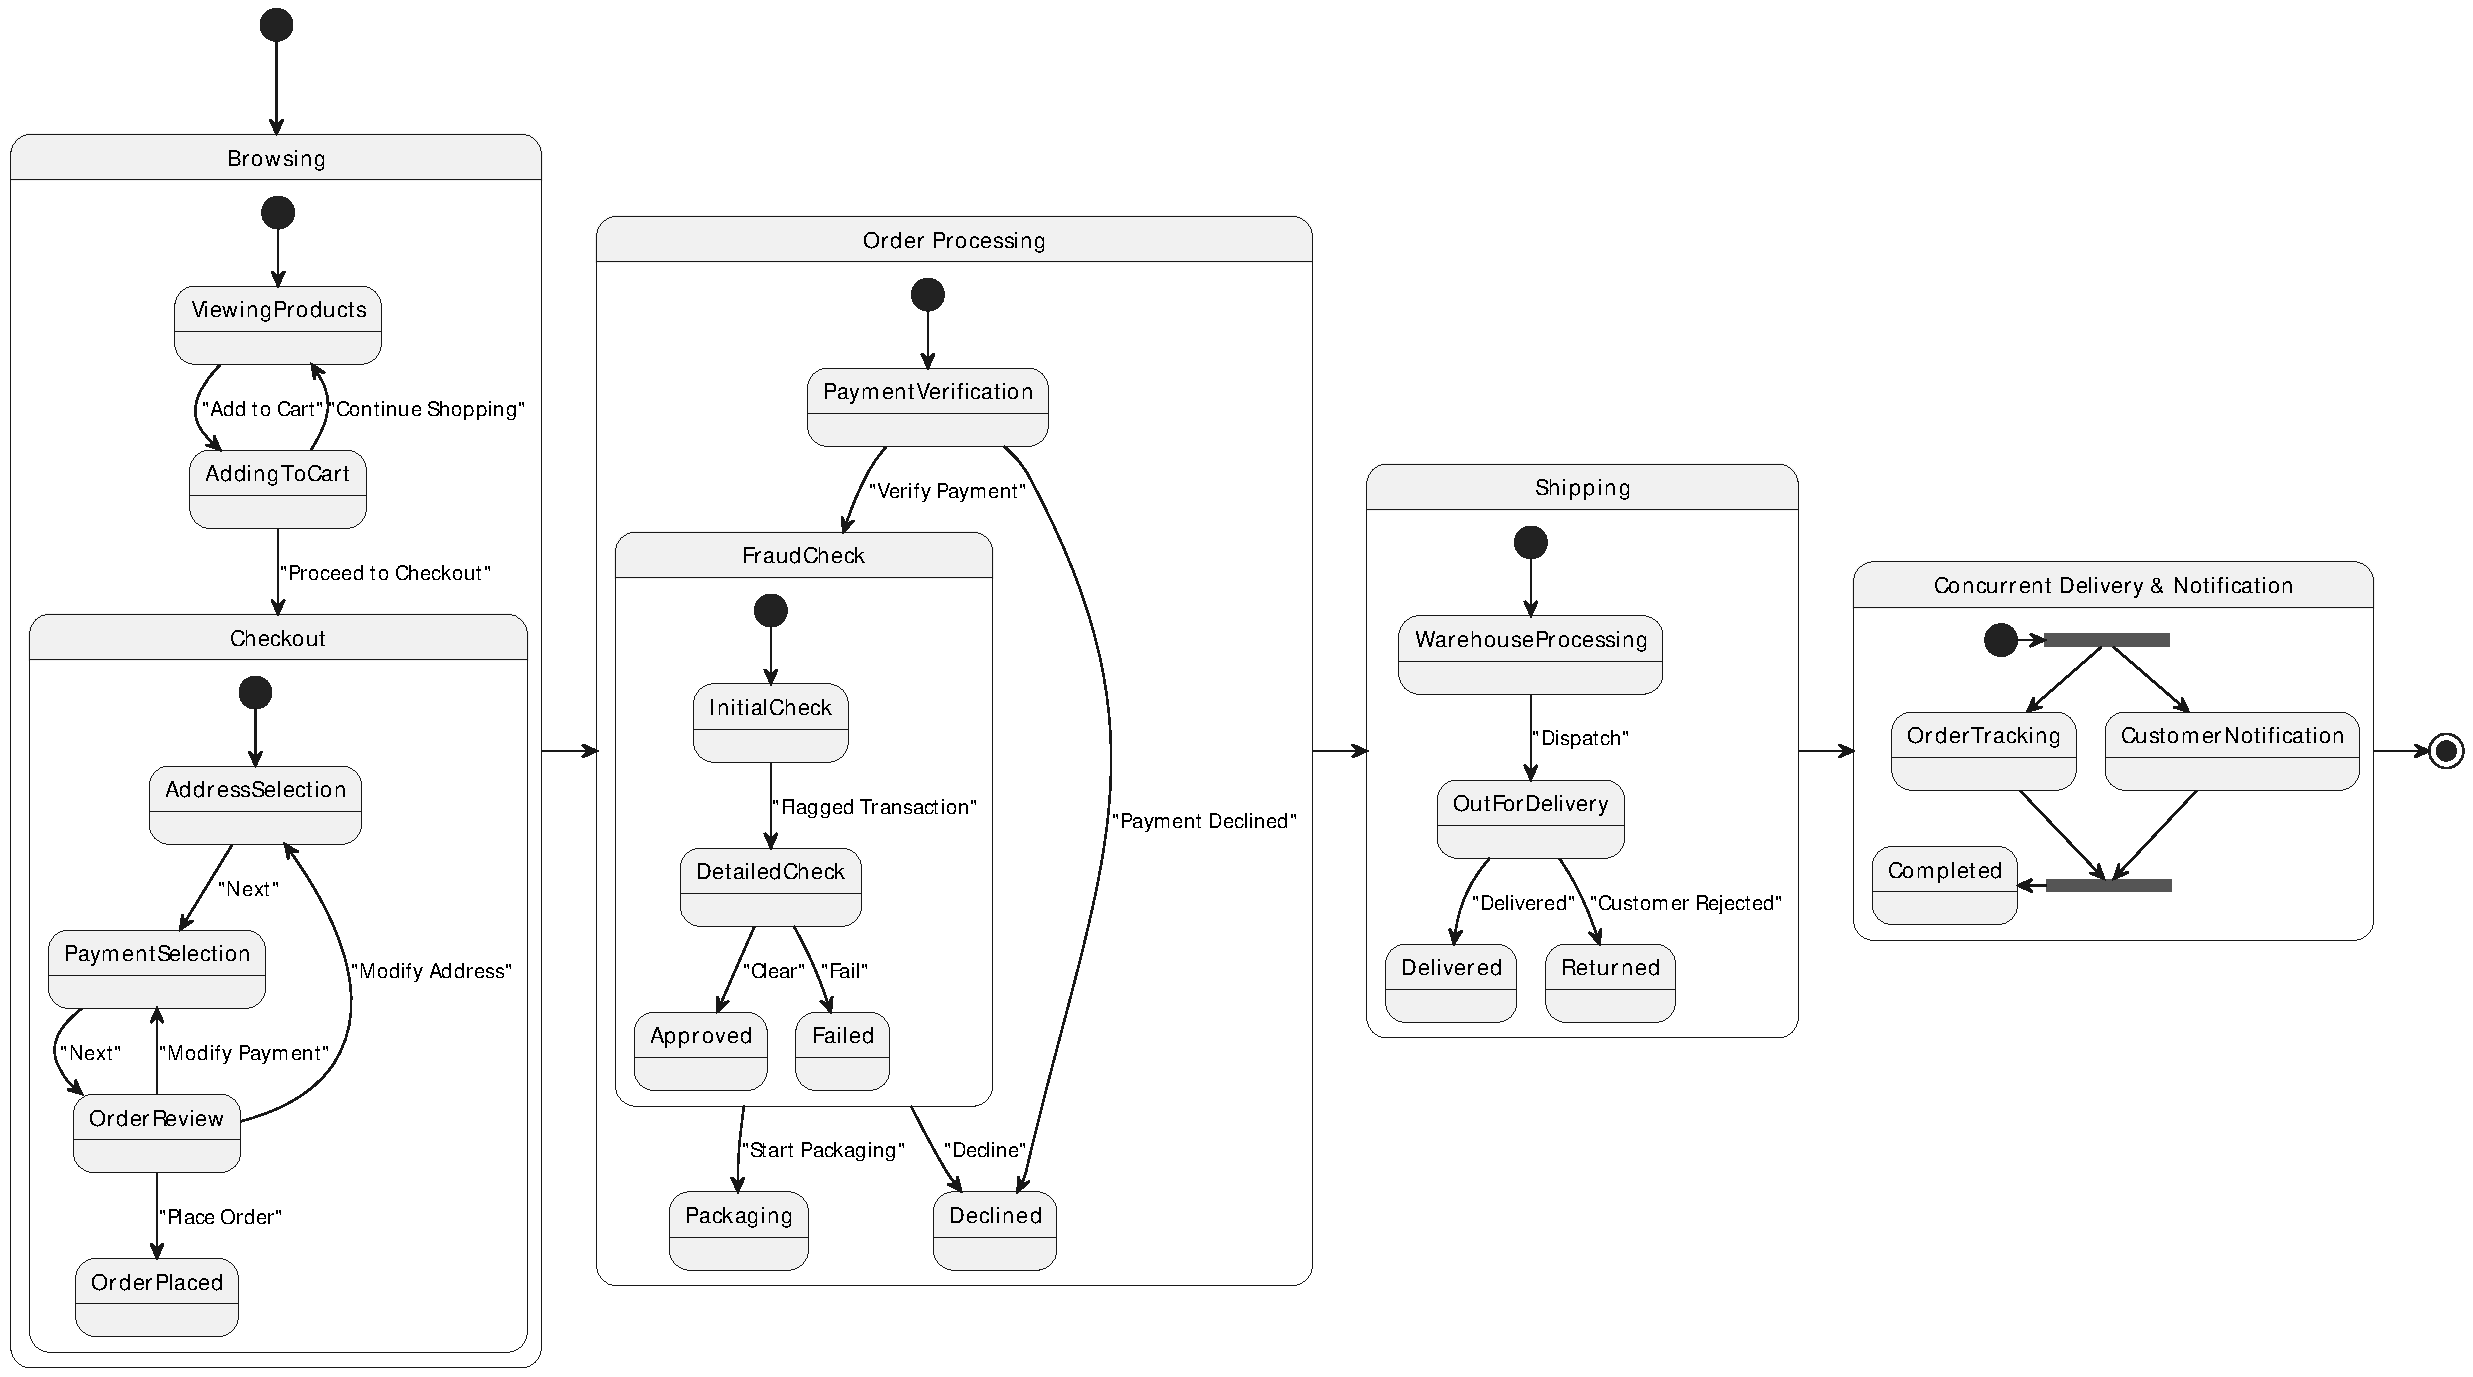
\includegraphics[width=\textwidth]{../figures/out/statechart_diagram}
	\caption{Statechart diagram and its features}
	\label{fig:statechart_diagram}
\end{figure}

\begin{lstlisting}[language=puml, caption={Statechart Diagram for E-Commerce Order Processing}]
	@startuml
	
	[*] --> Browsing
	
	state Browsing {
		[*] --> ViewingProducts
		ViewingProducts --> AddingToCart : "Add to Cart"
		AddingToCart --> ViewingProducts : "Continue Shopping"
		AddingToCart --> Checkout : "Proceed to Checkout"
	}
	
	state Checkout {
		[*] --> AddressSelection
		AddressSelection --> PaymentSelection : "Next"
		PaymentSelection --> OrderReview : "Next"
		OrderReview --> OrderPlaced : "Place Order"
		OrderReview --> AddressSelection : "Modify Address"
		OrderReview --> PaymentSelection : "Modify Payment"
	}
	
	Browsing -r-> OrderProcessing
	
	state "Order Processing" as OrderProcessing {
		[*] --> PaymentVerification
		PaymentVerification --> FraudCheck : "Verify Payment"
		PaymentVerification --> Declined : "Payment Declined"
		
		state FraudCheck {
			[*] --> InitialCheck
			InitialCheck --> DetailedCheck : "Flagged Transaction"
			DetailedCheck --> Approved : "Clear"
			DetailedCheck --> Failed : "Fail"
		}
		
		FraudCheck --> Declined: "Decline"
		FraudCheck --> Packaging : "Start Packaging"
	}
	
	OrderProcessing -r-> Shipping
	
	state "Shipping" as Shipping {
		[*] --> WarehouseProcessing
		WarehouseProcessing --> OutForDelivery : "Dispatch"
		OutForDelivery --> Delivered : "Delivered"
		OutForDelivery --> Returned : "Customer Rejected"
	}
	
	Shipping -r-> DeliveryProcess
	
	state "Concurrent Delivery & Notification" as DeliveryProcess {
		
		state fork_state <<fork>>
		[*] -r-> fork_state 
		fork_state --> OrderTracking
		fork_state --> CustomerNotification
		
		state join_state <<join>>
		OrderTracking --> join_state
		CustomerNotification --> join_state
		Completed <-- join_state
		
	}
	
	DeliveryProcess -r-> [*]
	
	@enduml
\end{lstlisting}


\subsection{Keadaan dan Transisi}
Dalam statechart diagram, sistem direpresentasikan sebagai kumpulan keadaan (state) yang berubah berdasarkan transisi. Setiap keadaan merepresentasikan kondisi tertentu yang dapat ditempati oleh suatu entitas dalam sistem. Transisi antar keadaan ditentukan oleh suatu peristiwa atau aksi. 

Dalam contoh diagram ini, sistem pemesanan e-commerce dimulai dari keadaan \texttt{Browsing}, di mana pengguna dapat menjelajahi produk, menambahkan produk ke dalam keranjang, dan melanjutkan ke proses checkout. Transisi dari \texttt{Browsing} ke \texttt{Checkout} terjadi ketika pengguna memilih untuk melakukan pembelian.

\begin{lstlisting}[language=puml]
	[*] --> Browsing
	Browsing {
		[*] --> ViewingProducts
		ViewingProducts --> AddingToCart : "Add to Cart"
		AddingToCart --> ViewingProducts : "Continue Shopping"
		AddingToCart --> Checkout : "Proceed to Checkout"
	}
\end{lstlisting}

\subsection{Keadaan Tersusun (Composite State)}
Statechart diagram mendukung keadaan tersusun (composite state) yang memungkinkan representasi keadaan yang lebih kompleks. Dalam contoh ini, \texttt{Order Processing} dan \texttt{FraudCheck} adalah contoh composite state, yang masing-masing memiliki sub-state di dalamnya. Composite state memungkinkan sistem untuk menggambarkan proses yang lebih terstruktur, seperti verifikasi pembayaran sebelum pesanan dapat diproses lebih lanjut.

\begin{lstlisting}[language=puml]
	state "Order Processing" as OrderProcessing {
		[*] --> PaymentVerification
		PaymentVerification --> FraudCheck : "Verify Payment"
		
		state FraudCheck {
			[*] --> InitialCheck
			InitialCheck --> DetailedCheck : "Flagged Transaction"
			DetailedCheck --> Approved : "Clear"
			DetailedCheck --> Failed : "Fail"
		}
		
		FraudCheck --> Packaging : "Start Packaging"
	}
\end{lstlisting}

\subsection{Transisi Bersyarat dan Penanganan Kesalahan}
Statechart diagram memungkinkan penggunaan transisi bersyarat untuk menangani keputusan logis dalam suatu sistem. Dalam proses pemesanan ini, setelah pembayaran diverifikasi, sistem melakukan pemeriksaan keamanan melalui \texttt{FraudCheck}. Jika transaksi ditandai sebagai mencurigakan, sistem melakukan pemeriksaan lebih lanjut. Jika transaksi tidak valid, sistem akan menolak pembayaran dan mengembalikan pengguna ke status \texttt{Declined}. Sebaliknya, jika transaksi valid, sistem akan melanjutkan ke proses pengemasan.

\begin{lstlisting}[language=puml]
	PaymentVerification --> FraudCheck : "Verify Payment"
	FraudCheck --> Declined : "Decline"
	FraudCheck --> Packaging : "Start Packaging"
\end{lstlisting}

\subsection{Fork dan Join untuk Eksekusi Paralel}
Dalam beberapa proses, terdapat aktivitas yang dapat berjalan secara paralel. Statechart diagram memungkinkan penggunaan \texttt{fork} dan \texttt{join} untuk merepresentasikan eksekusi bersamaan. Dalam contoh ini, setelah pesanan dikirim, sistem menjalankan dua proses paralel, yaitu pelacakan pesanan (\texttt{OrderTracking}) dan pemberitahuan pelanggan (\texttt{CustomerNotification}). Kedua proses ini berjalan secara independen dan akan digabung kembali dalam \texttt{join\_state} sebelum sistem menyelesaikan proses pengiriman.

\begin{lstlisting}[language=puml]
	state "Concurrent Delivery & Notification" as DeliveryProcess {
		
		state fork_state <<fork>>
		[*] -r-> fork_state 
		fork_state --> OrderTracking
		fork_state --> CustomerNotification
		
		state join_state <<join>>
		OrderTracking --> join_state
		CustomerNotification --> join_state
		Completed <-- join_state
	}
\end{lstlisting}

\subsection{Keadaan Awal dan Akhir}
Statechart diagram memiliki simbol keadaan awal dan akhir yang ditandai dengan \texttt{[*]}. Keadaan awal menunjukkan titik masuk sistem, sedangkan keadaan akhir menunjukkan titik keluarnya sistem. Dalam contoh diagram ini, keadaan awal dimulai dari \texttt{Browsing}, dan sistem berakhir setelah pesanan selesai diproses di keadaan \texttt{Completed}.

\begin{lstlisting}[language=puml]
	[*] --> Browsing
	Completed --> [*]
\end{lstlisting}

Statechart diagram sangat berguna untuk merepresentasikan perubahan keadaan dalam sistem yang memiliki alur kerja kompleks, seperti proses pemesanan dalam e-commerce. Dengan menggunakan elemen-elemen seperti \textbf{keadaan tersusun (composite state)}, \textbf{transisi bersyarat}, \textbf{fork dan join untuk eksekusi paralel}, serta \textbf{eadaan awal dan akhir}, diagram ini memberikan gambaran yang jelas mengenai bagaimana suatu sistem merespons berbagai kejadian selama siklus hidupnya. Dengan pemodelan ini, pengembang dapat lebih mudah memahami bagaimana sistem bekerja, mendeteksi potensi masalah, dan mengoptimalkan proses bisnis sebelum implementasi dilakukan.


\section{Use Case Diagram}

Use case diagram merupakan salah satu diagram perilaku dalam Unified Modeling Language (UML) yang digunakan untuk merepresentasikan interaksi antara pengguna (aktor) dan sistem. Diagram ini menunjukkan berbagai fungsi yang tersedia dalam sistem dan bagaimana aktor berinteraksi dengan masing-masing fungsi tersebut. 

Pada contoh ini, digunakan use case diagram untuk menggambarkan proses utama dalam sistem e-commerce, mencakup aktivitas pelanggan dalam mencari produk, menambahkan ke keranjang, melakukan checkout, hingga pelacakan pesanan. Selain itu, diagram ini juga mencakup peran admin dalam mengelola pesanan, menghasilkan laporan, serta peran sistem eksternal seperti gateway pembayaran.

\begin{figure}[ht]
	\centering
	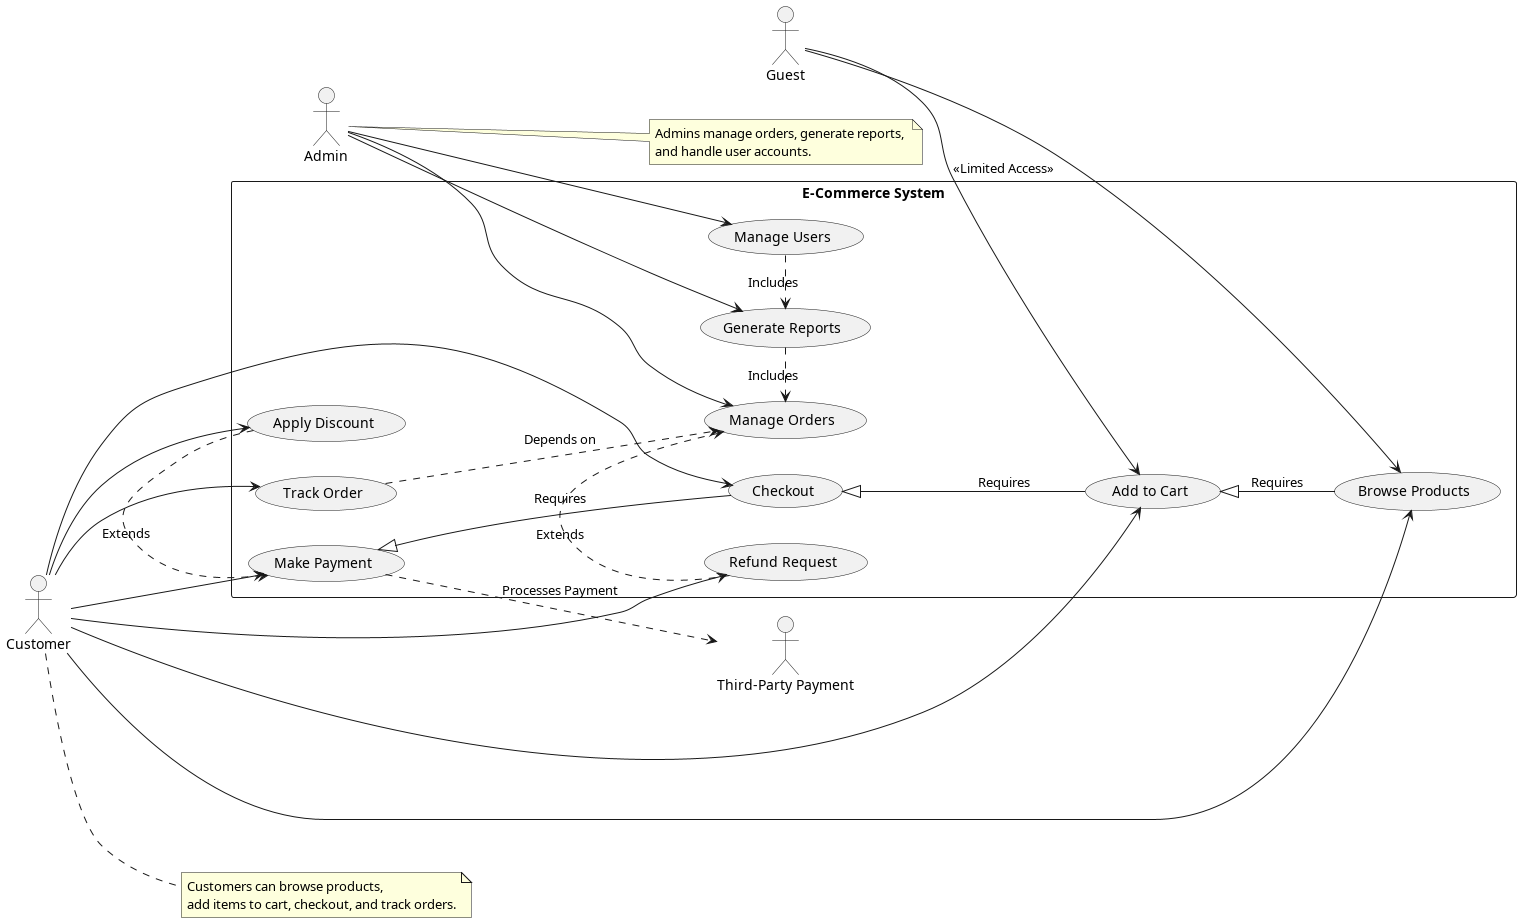
\includegraphics[width=\textwidth]{../figures/out/usecase_diagram}
	\caption{Use Case Diagram for E-Commerce System}
	\label{fig:usecase_diagram}
\end{figure}

\begin{lstlisting}[language=puml, caption={Use Case Diagram for E-Commerce System}]
	@startuml
	
	' skinparam linetype polyline
	' skinparam linetype ortho
	left to right direction
	' Define actors
	actor Customer
	actor Guest
	actor Admin
	actor "Third-Party Payment" as PaymentGateway
	
	' Define system boundary
	rectangle "E-Commerce System" {
		
		' Primary use cases
		usecase "Browse Products" as UC1
		usecase "Add to Cart" as UC2
		usecase "Checkout" as UC3
		usecase "Make Payment" as UC4
		usecase "Track Order" as UC5
		usecase "Manage Orders" as UC6
		usecase "Refund Request" as UC7
		usecase "Apply Discount" as UC8
		usecase "Generate Reports" as UC9
		usecase "Manage Users" as UC10
		
		' Relationships
		UC2 <|-- UC1 : "Requires"
		UC3 <|-- UC2 : "Requires"
		UC4 <|-- UC3 : "Requires"
		
		UC4 ..> PaymentGateway : "Processes Payment"
		UC5 ..> UC6 : "Depends on"
		UC7 .> UC6 : "Extends"
		UC8 .> UC4 : "Extends"
		
		' Admin-specific use cases
		UC9 .> UC6 : "Includes"
		UC10 .> UC9 : "Includes"
	}
	
	' Assign actors to use cases
	Customer --> UC1
	Customer --> UC2
	Customer --> UC3
	Customer --> UC4
	Customer --> UC5
	Customer --> UC7
	Customer --> UC8
	
	Guest --> UC1
	Guest --> UC2 : "<<Limited Access>>"
	
	Admin --> UC6
	Admin --> UC9
	Admin --> UC10
	
	' Notes
	note right of Customer
	Customers can browse products,
	add items to cart, checkout, and track orders.
	end note
	
	note right of Admin
	Admins manage orders, generate reports, 
	and handle user accounts.
	end note
	
	@enduml
\end{lstlisting}


\subsection{Aktor dalam Use Case Diagram}
Aktor merupakan entitas eksternal yang berinteraksi dengan sistem untuk mencapai tujuan tertentu. Dalam contoh ini, terdapat empat aktor utama:
\begin{enumerate}
	\item \textbf{Customer}, yaitu pengguna utama yang melakukan pembelian produk.
	\item \textbf{Guest}, yaitu pengguna yang dapat menjelajahi produk tetapi memiliki akses terbatas.
	\item \textbf{Admin}, yang bertanggung jawab untuk mengelola pesanan, pelanggan, dan laporan.
	\item \textbf{Third-Party Payment}, yaitu sistem eksternal yang menangani transaksi pembayaran.
\end{enumerate}

Aktor-aktor ini direpresentasikan dengan simbol stick figure dan memiliki garis koneksi ke berbagai use case dalam sistem.

\begin{lstlisting}[language=puml]
	actor Customer
	actor Guest
	actor Admin
	actor "Third-Party Payment" as PaymentGateway
\end{lstlisting}

\subsection{Use Case dan Relasi}
Use case merepresentasikan fungsi atau layanan yang tersedia dalam sistem. Dalam sistem e-commerce ini, beberapa use case utama yang tersedia meliputi:
\begin{enumerate}
	\item \textbf{Browse Products}: Pelanggan atau tamu dapat melihat daftar produk yang tersedia.
	\item \textbf{Add to Cart}: Pelanggan dapat menambahkan produk ke keranjang belanja.
	\item \textbf{Checkout}: Pelanggan melakukan proses pembayaran.
	\item \textbf{Make Payment}: Transaksi pembayaran diproses melalui gateway pembayaran eksternal.
	\item \textbf{Track Order}: Pelanggan dapat melacak status pengiriman pesanan mereka.
	\item \textbf{Manage Orders}: Admin dapat mengelola pesanan pelanggan.
	\item \textbf{Refund Request}: Pelanggan dapat mengajukan permintaan pengembalian dana jika diperlukan.
	\item \textbf{Apply Discount}: Sistem dapat menerapkan diskon saat pembayaran dilakukan.
	\item \textbf{Generate Reports}: Admin dapat menghasilkan laporan terkait transaksi dan aktivitas pengguna.
	\item \textbf{Manage Users}: Admin dapat mengelola informasi pengguna dalam sistem.
\end{enumerate}

Setiap use case direpresentasikan dengan elips dalam diagram, dan aktor yang terkait memiliki koneksi ke use case yang mereka gunakan.

\begin{lstlisting}[language=puml]
	rectangle "E-Commerce System" {
		usecase "Browse Products" as UC1
		usecase "Add to Cart" as UC2
		usecase "Checkout" as UC3
		usecase "Make Payment" as UC4
		usecase "Track Order" as UC5
		usecase "Manage Orders" as UC6
		usecase "Refund Request" as UC7
		usecase "Apply Discount" as UC8
		usecase "Generate Reports" as UC9
		usecase "Manage Users" as UC10
	}
\end{lstlisting}

\subsection{Relasi dalam Use Case Diagram}
Dalam use case diagram, terdapat beberapa jenis hubungan yang menghubungkan use case satu dengan lainnya:
\begin{enumerate}
	\item \textbf{Generalization (\texttt{<|--})}: Digunakan untuk menunjukkan bahwa satu use case merupakan bentuk spesifik dari use case lainnya. Contohnya, \texttt{Add to Cart} adalah bagian dari \texttt{Browse Products}, sedangkan \texttt{Checkout} bergantung pada \texttt{Add to Cart}.
	\begin{lstlisting}[language=puml]
		UC2 <|-- UC1 : "Requires"
		UC3 <|-- UC2 : "Requires"
		UC4 <|-- UC3 : "Requires"
	\end{lstlisting}
	
	\item \textbf{Include (\texttt{.>})}: Digunakan untuk menunjukkan bahwa satu use case selalu memanggil use case lainnya sebagai bagian dari prosesnya. Misalnya, \texttt{Generate Reports} mengandung bagian dari \texttt{Manage Orders} dan \texttt{Manage Users}.
	\begin{lstlisting}[language=puml]
		UC9 .> UC6 : "Includes"
		UC10 .> UC9 : "Includes"
	\end{lstlisting}
	
	\item \textbf{Extend (\texttt{..>})}: Menunjukkan bahwa use case dapat memperluas fungsi use case lain dalam kondisi tertentu. Sebagai contoh, \texttt{Refund Request} memperpanjang \texttt{Manage Orders} karena tidak semua pesanan akan mengalami pengembalian dana.
	\begin{lstlisting}[language=puml]
		UC7 ..> UC6 : "Extends"
		UC8 ..> UC4 : "Extends"
	\end{lstlisting}
\end{enumerate}

\subsection{Hubungan Aktor dengan Use Case}
Setiap aktor dalam sistem memiliki hubungan dengan satu atau lebih use case. Pelanggan memiliki akses ke hampir semua fitur utama, sementara tamu hanya memiliki akses terbatas. Admin memiliki akses ke fitur manajemen sistem.

\begin{lstlisting}[language=puml]
	Customer --> UC1
	Customer --> UC2
	Customer --> UC3
	Customer --> UC4
	Customer --> UC5
	Customer --> UC7
	Customer --> UC8
	
	Guest --> UC1
	Guest --> UC2 : "<<Limited Access>>"
	
	Admin --> UC6
	Admin --> UC9
	Admin --> UC10
\end{lstlisting}

\subsection{Pemberian Catatan pada Diagram}
PlantUML memungkinkan penambahan catatan untuk memberikan informasi tambahan dalam diagram. Dalam contoh ini, terdapat catatan yang menjelaskan peran masing-masing aktor dalam sistem.

\begin{lstlisting}[language=puml]
	note right of Customer
	Customers can browse products,
	add items to cart, checkout, and track orders.
	end note
	
	note right of Admin
	Admins manage orders, generate reports, 
	and handle user accounts.
	end note
\end{lstlisting}

Use case diagram memberikan gambaran bagaimana aktor berinteraksi dengan sistem melalui berbagai fungsi yang tersedia. Dalam contoh ini, sistem e-commerce memiliki berbagai aktor seperti pelanggan, tamu, admin, dan sistem pembayaran eksternal yang berinteraksi dengan beberapa use case. Dengan menggunakan hubungan seperti \textbf{generalization, include, dan extend}, diagram ini memberikan representasi yang jelas mengenai bagaimana fitur dalam sistem saling berkaitan.

Use case diagram sangat berguna dalam tahap perancangan perangkat lunak karena dapat membantu pemangku kepentingan dalam memahami bagaimana pengguna berinteraksi dengan sistem sebelum implementasi dilakukan.

\section{Referensi}
Untuk pembelajaran lebih mendalam mengenai UML, silahkan kunjungi tautan berikut: \url{https://www.uml-diagrams.org/}.
